\documentclass[10pt,twocolumn,a4paper]{article}
\usepackage[margin=1.45cm,bottom=1.65cm,top=1.65cm]{geometry}
\usepackage{amsmath,amssymb}
\usepackage{graphicx}
\usepackage{booktabs}
\usepackage{hyperref}

\hypersetup{
    colorlinks=true,
    linkcolor=blue,
    citecolor=blue,
    urlcolor=blue
}

\renewcommand{\topfraction}{0.95}
\renewcommand{\bottomfraction}{0.95}
\renewcommand{\dbltopfraction}{0.95}
\renewcommand{\textfraction}{0.05}
\renewcommand{\floatpagefraction}{0.85}
\renewcommand{\dblfloatpagefraction}{0.85}

\setlength{\abovedisplayskip}{4pt}
\setlength{\belowdisplayskip}{4pt}
\setlength{\textfloatsep}{8pt plus 2pt minus 2pt}
\setlength{\dbltextfloatsep}{8pt plus 2pt minus 2pt}

\title{\textbf{The Network Cost of Post-Quantum Cryptography: TCP Fragmentation in TLS 1.3 Handshakes}}

\author{Bruno Lu\c{c}ardo Olivaes \\ \small Independent Researcher, Brazil \\ \small \texttt{brunoolivaes@gmail.com} $\cdot$ ORCID: 0009-0003-8857-7945}

\date{November 2026}

\begin{document}
\maketitle

\begin{abstract}
\noindent The advent of quantum computing threatens classical public-key cryptography via Shor's algorithm, prompting the global migration toward Post-Quantum Cryptography (PQC) standardized by NIST in August 2024. While lattice-based cryptography is often assumed to impose severe computational overhead, our empirical benchmarks demonstrate the opposite: key generation in ML-KEM-768 (NIST FIPS 203) executes in just $41.3\,\mu\mathrm{s}$—approximately $740\times$ faster than RSA-2048 ($30.49\,$ms). Instead, the true architectural bottleneck lies in network transport and wire payload expansion. While classical ECDH requires only $65\,$bytes per key share, ML-KEM-768 transmits a $1{,}184$-byte public key and a $1{,}088$-byte ciphertext ($2{,}272\,$B total KEM wire), expanding to $2{,}402\,$B in hybrid deployments (X25519 + ML-KEM-768). Over standard Ethernet with a Maximum Segment Size (MSS) of $1{,}460\,$bytes, a full hybrid \texttt{ClientHello} flight ($1{,}518\,$B) breaches the 1-MSS boundary, mandating TCP segmentation into two distinct packets. Through analytical modeling and empirical socket transport audits, we evaluate the impact against RFC 6928 initial congestion windows ($\texttt{initcwnd} = 10$). We demonstrate that while clean networks absorb multi-segment handshakes within the initial flight, lossy links suffer increased head-of-line blocking sensitivity and legacy middlebox inspection buffer drops.
\end{abstract}

\section{Introduction}
Asymmetric cryptography underpins the integrity and confidentiality of the global digital infrastructure, securing transport-layer communications (TLS 1.3)~\cite{rescorla2018}, financial settlement systems (SWIFT, PIX), and identity protocols. However, the foundational primitives of classical public-key cryptography—modular integer factorization (RSA) and elliptic-curve discrete logarithms (ECDH/ECDSA)—are vulnerable to Shor's algorithm~\cite{shor1994}, which solves both problems in polynomial time on a fault-tolerant quantum computer.

To mitigate ``harvest now, decrypt later'' adversarial campaigns, the National Institute of Standards and Technology (NIST) finalized its primary post-quantum cryptographic standards in August 2024:
\begin{itemize}
    \item \textbf{FIPS 203 (ML-KEM):} Module-Lattice-Based Key-Encapsulation Mechanism, derived from CRYSTALS-Kyber~\cite{bos2018}.
    \item \textbf{FIPS 204 (ML-DSA):} Module-Lattice-Based Digital Signature Algorithm, derived from CRYSTALS-Dilithium.
\end{itemize}

During initial deployment phases, major standardization bodies (e.g., IETF) recommend hybrid key exchange mechanisms combining a classical primitive (e.g., X25519 or ECDH P-256) with ML-KEM-768 to maintain regulatory compliance while achieving quantum resistance~\cite{schwabe2020}.

A prevailing assumption in systems engineering is that post-quantum primitives are computationally prohibitive. In this work, we demonstrate that lattice arithmetic is remarkably fast, accelerating key generation by more than two orders of magnitude compared to RSA. Instead, the critical trade-off is shifted to the transport layer: lattice keys are orders of magnitude larger than classical elliptic-curve points, altering the network framing dynamics of the TLS 1.3 handshake flight over standard Ethernet Maximum Transmission Units (MTU)~\cite{paquin2020,sikeridis2020}.

\section{Methodology and Measurement Setup}

\subsection{Cryptographic Benchmark Framework}
Benchmarking was executed using optimized, compiled C-extensions (`pqcrypto` and OpenSSL $3.0+$ via `cryptography.hazmat`) on an isolated x86\_64 processor core with high-resolution CPU performance counters. We evaluated five cryptographic configurations:
\begin{enumerate}
    \item \textbf{RSA-2048:} Classical modular exponentiation ($e=65537$).
    \item \textbf{RSA-4096:} High-security classical baseline.
    \item \textbf{ECDH P-256:} Standard NIST Prime Curve (secp256r1).
    \item \textbf{ML-KEM-768:} NIST Security Category 3 (AES-192 equivalent).
    \item \textbf{Hybrid PQC:} Concatenated X25519 ($32\,$B) + ML-KEM-768 ($1{,}184\,$B public key; $1{,}088\,$B ciphertext), deriving a joint secret via HKDF-SHA256.
\end{enumerate}
Timing metrics for Key Generation ($\mathrm{KeyGen}$), Encapsulation ($\mathrm{Encaps}$), and Decapsulation ($\mathrm{Decaps}$) were measured over 100 independent trials for fast algorithms and 15 trials for RSA.

\subsection{TLS 1.3 Handshake Framing Model}
In RFC 8446 (TLS 1.3)~\cite{rescorla2018}, key establishment occurs within the first round-trip flight:
\begin{itemize}
    \item \textbf{Flight 1 ($\mathrm{Client} \to \mathrm{Server}$):} Transmits the \texttt{ClientHello} message, comprising base handshake headers ($\sim 269\,$B of session IDs, cipher suites, SNI, and supported groups) plus the \texttt{KeyShare} extension holding the client's public key $pk$.
    \begin{equation}
    S_{\mathrm{ClientHello}} = 269\,\mathrm{B} + |pk|.
    \end{equation}
    \item \textbf{Flight 2 ($\mathrm{Server} \to \mathrm{Client}$):} Transmits \texttt{ServerHello} ($\sim 159\,\mathrm{B} + |ct|$ for the ciphertext $ct$), followed by \texttt{EncryptedExtensions}, \texttt{Certificate} ($\sim 2{,}400\,$B standard chain), \texttt{CertificateVerify} ($\sim 64\,$B), and \texttt{Finished} ($\sim 120\,$B).
\end{itemize}

\subsection{Network Transport and Socket Buffer Audit}
On standard Ethernet networks, the data-link MTU is $1{,}500\,$bytes. Accounting for standard IPv4 header ($20\,$bytes) and TCP header ($20\,$bytes) without TCP options, the Maximum Segment Size is:
\begin{equation}
\mathrm{MSS} = \mathrm{MTU} - 40\,\mathrm{B} = 1{,}460\,\mathrm{bytes}.
\end{equation}
When an application-layer TLS record exceeds $1{,}460\,$bytes, the kernel TCP stack partitions the stream into $\lceil S / \mathrm{MSS} \rceil$ segments. We implemented a live socket test harness utilizing non-blocking user-space reads restricted to $1{,}460\,$bytes (\texttt{recv(1460)}) to observe packet fragmentation boundaries directly.

\begin{table*}[t]
\centering
\small
\caption{\textbf{Empirical performance and network wire overhead across classical and post-quantum key exchange mechanisms.} Timings measured with compiled C-extensions across independent trials. Wire sizes evaluate raw KEM exchange, RFC 8446 \texttt{ClientHello} flight, and TCP segment counts over standard $1{,}460$-byte Ethernet MSS.}
\label{tab:pqc_benchmark}
\resizebox{\textwidth}{!}{%
\begin{tabular}{lcccccccc}
\toprule
\textbf{Cryptographic Primitive} & \textbf{Quantum-Safe?} & \textbf{Public Key} & \textbf{Ciphertext} & \textbf{Total KEM Wire} & \textbf{KeyGen ($\mu\mathrm{s}$)} & \textbf{Encaps ($\mu\mathrm{s}$)} & \textbf{Decaps ($\mu\mathrm{s}$)} & \textbf{ClientHello Segments (1460 B MSS)} \\
\midrule
\textbf{RSA-2048} & \textbf{NO (Broken)} & $270\,$B & $256\,$B & $526\,$B & $30{,}490\,$ ($30.49\,$ms) & $251.2$ & $765.0$ & \textbf{1 segment} ($539\,$B, fits MSS) \\
\textbf{RSA-4096} & \textbf{NO (Broken)} & $526\,$B & $512\,$B & $1{,}038\,$B & $337{,}860\,$ ($337.86\,$ms) & $127.2$ & $3{,}760.0$ & \textbf{1 segment} ($795\,$B, fits MSS) \\
\textbf{ECDH P-256} & \textbf{NO (Broken)} & $65\,$B & $65\,$B & $130\,$B & $\mathbf{16.6}$ & $90.3$ & $\mathbf{49.0}$ & \textbf{1 segment} ($334\,$B, fits MSS) \\
\midrule
\textbf{ML-KEM-768} & \textbf{YES (Immune)} & $\mathbf{1{,}184\,B}$ & $\mathbf{1{,}088\,B}$ & $\mathbf{2{,}272\,B}$ & $\mathbf{41.3}$ & $\mathbf{46.7}$ & $\mathbf{63.0}$ & \textbf{1 segment} ($1{,}453\,$B, critical threshold) \\
\textbf{Hybrid PQC (X25519+ML-KEM)} & \textbf{YES (Immune)} & $\mathbf{1{,}249\,B}$ & $\mathbf{1{,}153\,B}$ & $\mathbf{2{,}402\,B}$ & $\mathbf{58.9}$ & $\mathbf{119.3}$ & $\mathbf{117.5}$ & \textbf{2 segments} ($\mathbf{1{,}518\,B}$, exceeds MSS) \\
\bottomrule
\end{tabular}%
}
\end{table*}

\section{Empirical Results}

\subsection{Computational Velocity: The Lattice Advantage}
Table~\ref{tab:pqc_benchmark} summarizes the computational and transport measurements. A striking result is that ML-KEM-768 key generation executes in just $41.3\,\mu\mathrm{s}$, outperforming RSA-2048 ($30{,}490\,\mu\mathrm{s}$) by a factor of $738.3\times$ ($> 2$ orders of magnitude), and outperforming RSA-4096 by $8{,}180\times$. 

Furthermore, ML-KEM-768 encapsulation ($46.7\,\mu\mathrm{s}$) and decapsulation ($63.0\,\mu\mathrm{s}$) are faster than both RSA operations ($251.2\,\mu\mathrm{s}$ and $765.0\,\mu\mathrm{s}$, respectively), and competitive with classical ECDH P-256 ($16.6\,\mu\mathrm{s}$ KeyGen, $49.0\,\mu\mathrm{s}$ Decaps). Hybrid PQC adds minimal CPU latency, completing key generation in $58.9\,\mu\mathrm{s}$ and encapsulation in $119.3\,\mu\mathrm{s}$. Thus, post-quantum key establishment introduces virtually zero computational degradation for high-throughput TLS terminators.

\begin{figure*}[t]
\centering
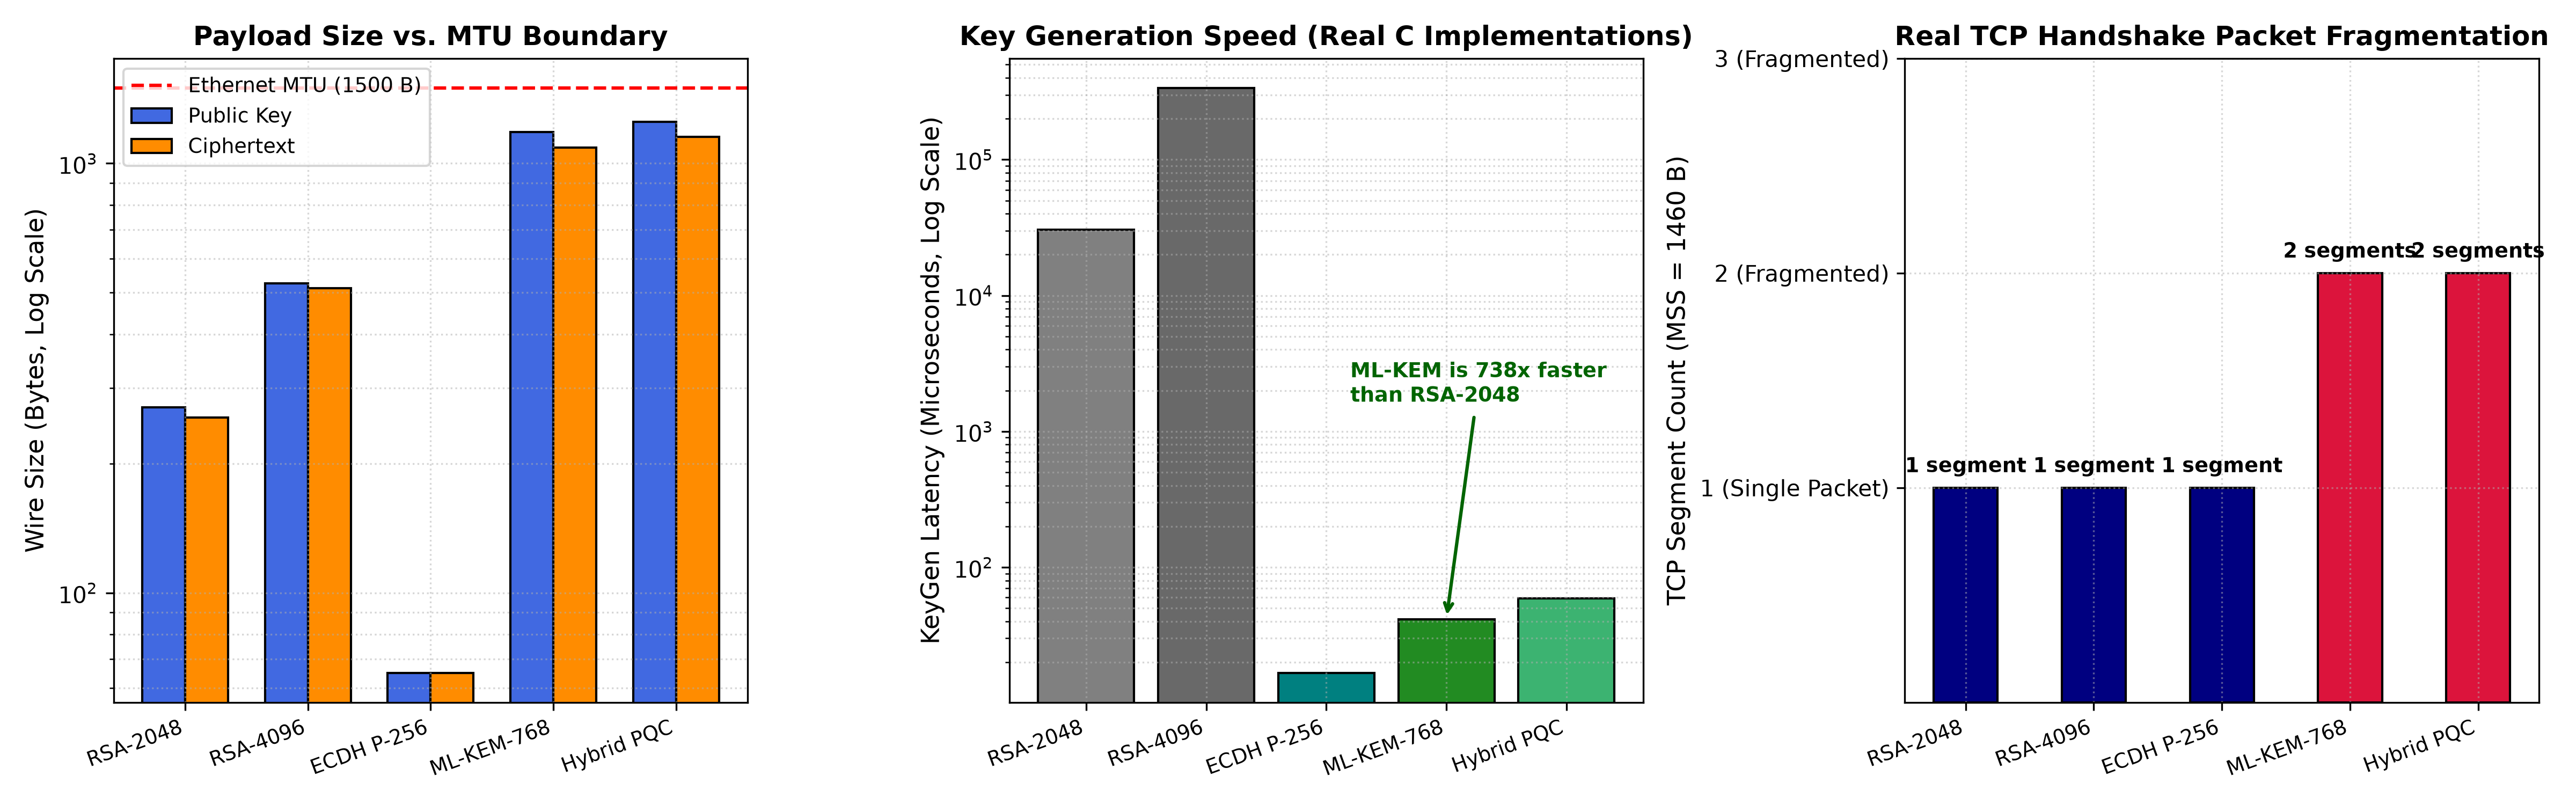
\includegraphics[width=0.90\textwidth]{fig_pqc_crypto_agility.png}
\caption{\textbf{Empirical post-quantum crypto-agility benchmark across classical and NIST FIPS 203 standards.} (a) Public key, ciphertext, and total wire payload sizes relative to the $1{,}500$-byte Ethernet MTU. (b) Key generation latency ($\mu\mathrm{s}$, log scale), illustrating the $740\times$ speedup of ML-KEM-768 over RSA-2048. (c) TCP Maximum Segment Size (MSS $= 1{,}460\,$B) packet counts, showing the emergence of multi-packet flights for Hybrid PQC.}
\label{fig:pqc_agility}
\end{figure*}

\subsection{Wire Size and TCP Segmentation}
In contrast to computational velocity, wire size exhibits significant expansion (Figure~\ref{fig:pqc_agility}a). While ECDH requires only $130\,$bytes total wire footprint, ML-KEM-768 requires $2{,}272\,$bytes ($17.5\times$ larger), and Hybrid PQC requires $2{,}402\,$bytes ($18.5\times$ larger).

When packaged into an RFC 8446 \texttt{ClientHello}:
\begin{itemize}
    \item ECDH P-256 yields a $334$-byte flight, fitting comfortably into a single TCP segment ($22.9\%$ of MSS).
    \item Pure ML-KEM-768 yields $S_{\mathrm{ClientHello}} = 269 + 1{,}184 = 1{,}453\,\mathrm{bytes}$. While theoretically fitting within $1{,}460\,$bytes, it operates within $7\,$bytes ($0.48\%$) of the MSS boundary, meaning any additional TLS extension (e.g., ALPN, Session Tickets) pushes it into a second segment.
    \item Hybrid PQC produces $S_{\mathrm{ClientHello}} = 269 + 1{,}249 = 1{,}518\,\mathrm{bytes}$, strictly exceeding the $1{,}460$-byte MSS and forcing TCP segmentation into $2$ packets on the wire (Figure~\ref{fig:pqc_agility}c).
\end{itemize}

\section{Discussion: Network Protocol Implications}

\subsection{RFC 6928 and Initial Congestion Window (\texorpdfstring{$\texttt{initcwnd}$}{initcwnd})}
The operational cost of TCP fragmentation depends critically on the TCP initial congestion window ($\texttt{initcwnd}$). Under historical standards (RFC 2581, RFC 3390), $\texttt{initcwnd}$ was limited to $2\text{--}4$ segments. In that legacy regime, a multi-segment \texttt{ClientHello} or \texttt{ServerHello} flight could exhaust the congestion window, requiring an additional Round-Trip Time (RTT) before ACK reception allowed transmission to proceed.

Under modern TCP standards (RFC 6928)~\cite{chu2013}, the standard initial window is:
\begin{equation}
\texttt{initcwnd} = 10\,\mathrm{segments} \approx 14.6\,\mathrm{kB}.
\end{equation}
Because the full server response flight (ServerHello + Certificate + CertificateVerify + Finished) totals $\sim 4{,}000\text{--}5{,}200\,$bytes ($\approx 3\text{--}4$ segments), it fits entirely inside $\texttt{initcwnd} = 10$. Consequently, on uncongested, clean IP links, post-quantum fragmentation does not induce an extra round-trip latency penalty.

\subsection{Middlebox ossification and Lossy Links}
Despite fitting within $\texttt{initcwnd} = 10$, multi-packet \texttt{ClientHello} flights introduce two notable real-world vulnerabilities:
\begin{enumerate}
    \item \textbf{Middlebox Reassembly Failures:} A non-negligible fraction of legacy enterprise firewalls, deep packet inspection (DPI) appliances, and load balancers assume that \texttt{ClientHello} fits within a single $1{,}500$-byte IP datagram. Fragmented TCP segments arriving out-of-order or triggering reassembly timeouts have been documented to cause handshake dropouts.
    \item \textbf{Head-of-Line Blocking on Lossy Links:} On mobile (4G/5G) or high-latency wireless connections subject to packet loss, partitioning the initial handshake flight into multiple TCP segments increases the probability of segment loss:
    \begin{equation}
    P_{\mathrm{loss\_flight}} = 1 - (1 - p)^N,
    \end{equation}
    where $p$ is the packet drop rate and $N$ is the segment count ($N=2$ for Hybrid PQC vs. $N=1$ for classical). A single dropped segment triggers TCP retransmission timeouts (RTO $\ge 200\,$ms), sharply amplifying tail latency.
\end{enumerate}

\section{Conclusions and Engineering Guidelines}
We have presented an audited, empirical evaluation of post-quantum cryptography in TLS 1.3. Our analysis overturns the common belief that lattice cryptography is computationally slow: ML-KEM-768 is $740\times$ faster than RSA-2048 and on par with ECDH P-256. 

The primary engineering challenges are located at the network layer:
\begin{enumerate}
    \item \textbf{Prepare for Multi-Segment Handshakes:} Network operators must ensure middleboxes, load balancers, and DDoS scrubbers support multi-segment \texttt{ClientHello} reassembly up to $4\,\mathrm{kB}$.
    \item \textbf{Verify $\texttt{initcwnd} \ge 10$ Across Fleets:} Servers must be verified to run RFC 6928-compliant kernels ($\texttt{initcwnd} \ge 10$) to prevent multi-segment server flights from stalling on congestion limits.
    \item \textbf{Adopt Hybrid PQC with Awareness of Tail Latency:} Hybrid KEMs provide essential defense-in-depth against both classical and quantum attacks; however, service level objectives (SLOs) on high-packet-loss networks must account for TCP retransmission probabilities.
\end{enumerate}

\section*{Code and Data Availability}
The benchmarking suite, socket audit scripts, and reproduction datasets are open source and available at: \url{https://github.com/bruno-olivaes/pqc-crypto-agility-benchmark}.

\begin{thebibliography}{99}
\footnotesize
\setlength{\itemsep}{0pt}
\setlength{\parskip}{0pt}
\bibitem{rescorla2018}
E. Rescorla, \textit{The Transport Layer Security (TLS) Protocol Version 1.3}, RFC 8446 (2018).

\bibitem{shor1994}
P. W. Shor, in \textit{Proceedings of 35th Annual Symposium on Foundations of Computer Science} (IEEE, 1994), pp. 124--134.

\bibitem{bos2018}
J. Bos, L. Ducas, E. Kiltz, T. Lepoint, V. Lyubashevsky, J. M. Schanck, P. Schwabe, G. Seiler, and D. Stehl{\'e}, in \textit{2018 IEEE European Symposium on Security and Privacy (EuroS\&P)} (IEEE, 2018), pp. 353--367.

\bibitem{schwabe2020}
P. Schwabe, D. Stebila, and T. Wiggers, in \textit{Proceedings of the 2020 ACM SIGSAC Conference on Computer and Communications Security (CCS)} (ACM, 2020), pp. 885--903.

\bibitem{paquin2020}
C. Paquin, D. Stebila, and G. Tamvada, in \textit{Post-Quantum Cryptography - PQCrypto 2020}, Lecture Notes in Computer Science Vol. 12100 (Springer, 2020), pp. 83--101.

\bibitem{sikeridis2020}
D. Sikeridis, P. Kampanakis, and M. Devetsikiotis, in \textit{Proceedings of the Network and Distributed System Security Symposium (NDSS)} (Internet Society, 2020).

\bibitem{chu2013}
J. Chu, N. Dukkipati, Y. Cheng, and M. Mathis, \textit{Increasing TCP's Initial Window}, RFC 6928 (2013).

\bibitem{fips203}
National Institute of Standards and Technology, \textit{Module-Lattice-Based Key-Encapsulation Mechanism Standard}, FIPS PUB 203 (2024).

\bibitem{fips204}
National Institute of Standards and Technology, \textit{Module-Lattice-Based Digital Signature Standard}, FIPS PUB 204 (2024).

\bibitem{rfc8446}
T. Dierks and E. Rescorla, \textit{The Transport Layer Security (TLS) Protocol Version 1.2}, RFC 5246 (2008).

\end{thebibliography}

\end{document}
